\section{Optimal Fine-gained Pruning}\label{sec:pruning}



In this section, we introduce a leaf-level pruning step that improves the efficiency of fully dynamic kNN join maintenance on \dualtree. The new step uses low-dimensional point-to-point distance to prune visited points inside leaf nodes before their full-dimensional distances are computed.

We further develop a cost-aware analysis for choosing the optimal pruning dimensionality. The goal is to balance the additional cost of low-dimensional distance computation against the extra pruning power it provides, so that the dimensionality is selected systematically rather than heuristically.

\subsection{Residual false positives after non-leaf pruning on \dualtree}
The non-leaf pruning on \dualtree remains essential: it removes large unpromising regions early and is the main reason why exact kNN search and RkNN search can be made efficient in high dimensions. However, this pruning is performed at the cluster level. As the search descends to the leaf nodes, some visited clusters that were correctly retained at upper levels may still contain individual points that are already far enough from the query point to be pruned.

This residual effect comes from the cluster-level lower-bound tests used at non-leaf nodes. In both \deltatree and \hdrtree, the quantity $dist_{PC}(center(C_j), q)-radius_{PC}(C_j)$ is a lower bound, in the PCA space of the current tree level, on the distance between the search-originating point $q$ and every point in cluster $C_j$~\cite{cui2003contorting,yang2014continuous}. In the \deltatree part, this lower bound is compared with the current kNN pruning threshold $dist_{prune}$; in the \hdrtree part, it is compared with the cluster-side threshold $\dmknn(C_j)$. These tests are effective for deciding whether a cluster may still contain useful candidates, but once a cluster is retained, all of its member points survive to deeper levels.

As a result, a retained cluster can still contain point-level false positives. This happens when the point determining $radius_{PC}(C_j)$ lies on the far side of the search-originating point: the lower bound for the cluster is then pulled down, so the cluster-level test remains correct but conservative. The cluster as a whole must be kept, even though many other points inside it are already beyond the pruning threshold and need not survive to the leaf level. Figure \ref{fig:knn_error} and Figure \ref{fig:rknn_error} illustrate this effect for kNN search and RkNN search, respectively.

\begin{figure}[t]
    
    \hspace*{0.15cm}
    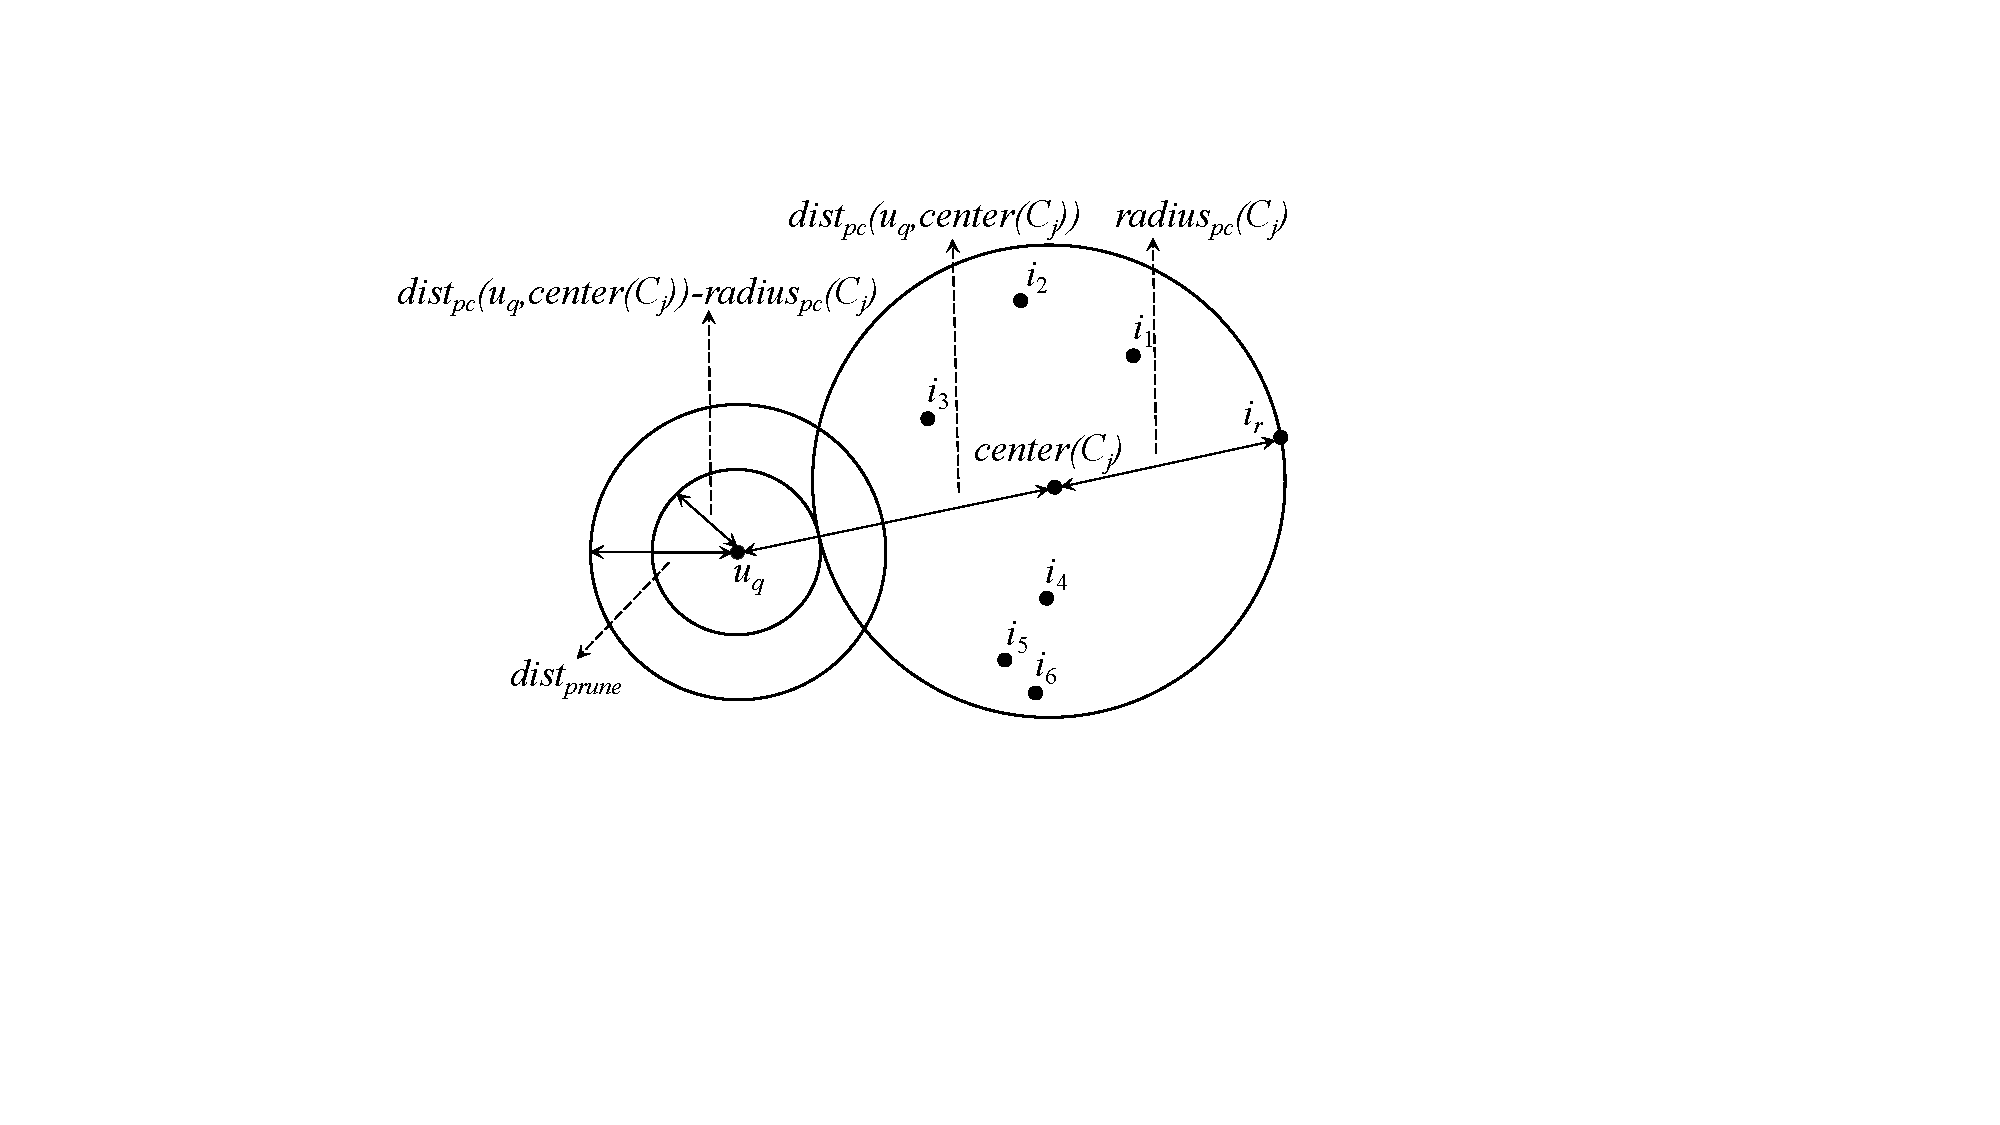
\includegraphics[width=0.41\textwidth]{Images/knn_error_11.pdf}
    \caption{Reservation of the remote data points that should be pruned in the kNN search process on \dualtree.}
    \label{fig:knn_error}
\end{figure}

\begin{figure}[t]
    \centering
    \hspace*{0.15cm}    
    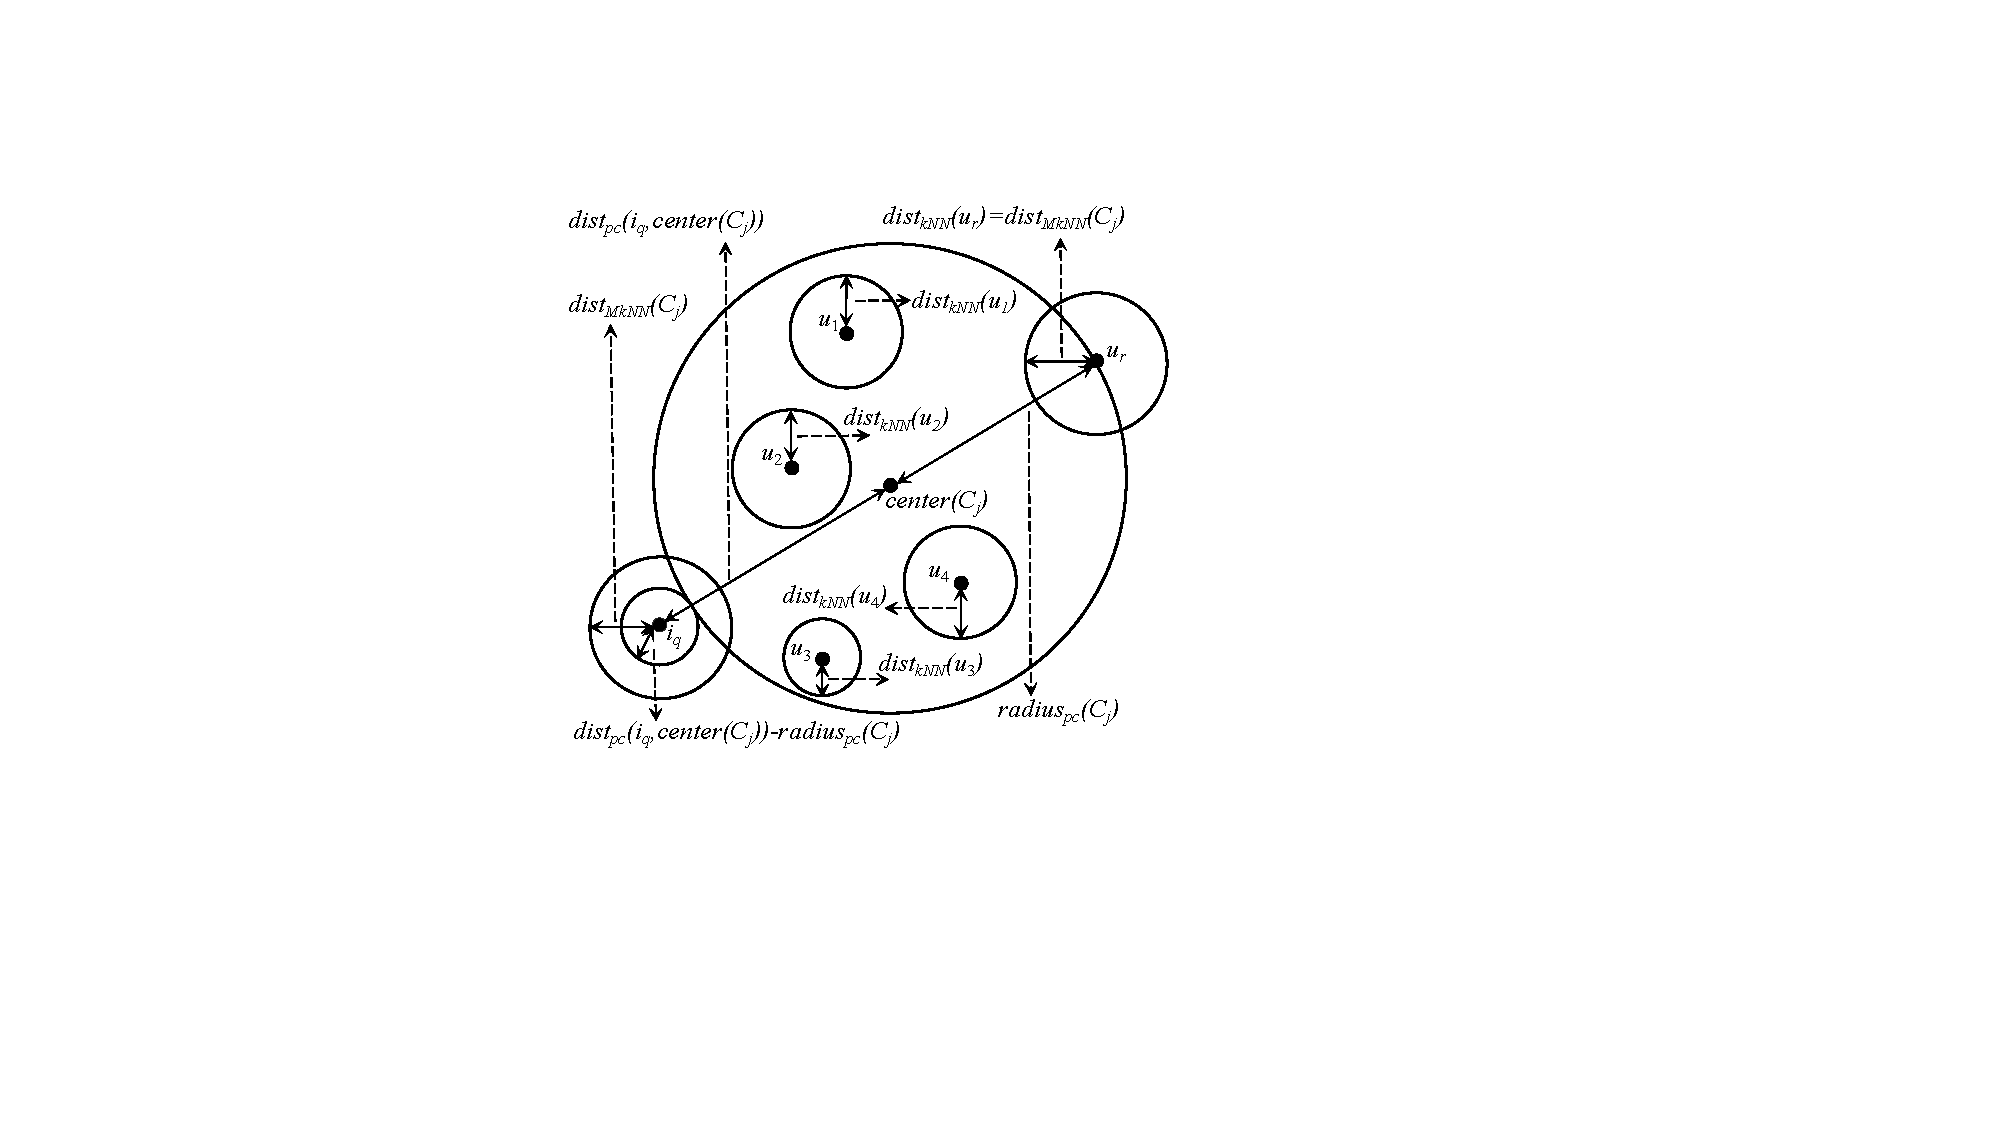
\includegraphics[width=0.4\textwidth]{Images/rknn_error_26.pdf}
    \caption{Reservation of the remote data points that should be pruned in the RkNN search process on \dualtree.}
    \label{fig:rknn_error}
\end{figure}


\begin{example}[False positive error in kNN search]
In Figure \ref{fig:knn_error}, a cluster $C_j$ at a non-leaf node in the \deltatree part of \dualtree is visited during kNN search for query point $u_q$. The cluster is retained because the lower-bound test $dist_{PC}(center(C_j), u_q)-radius_{PC}(C_j)<dist_{prune}$ holds. The far-side point $i_r$ determines the large value of $radius_{PC}(C_j)$ and keeps this lower bound below $dist_{prune}$. Nevertheless, every point in $C_j$ is actually farther from $u_q$ than $dist_{prune}$, so the cluster survives only because the test is applied to the cluster as a whole rather than to its member points.  
\label{example:false positive error in kNN Search}
\end{example}

\begin{example}[False positive error in RkNN search]
In Figure \ref{fig:rknn_error}, a cluster $C_j$ at a non-leaf node in the \hdrtree part of \dualtree is visited during RkNN search for query point $i_q$. The cluster is retained because the lower-bound test $dist_{PC}(center(C_j), i_q)-radius_{PC}(C_j)<\dmknn(C_j)$ holds. The far-side point $u_r$ determines the large value of $radius_{PC}(C_j)$ and keeps this lower bound below $\dmknn(C_j)$. Nevertheless, for every data point $u\in C_j$, the distance from $i_q$ to $u$ still exceeds $\dmknn(C_j)$, so no point in the cluster should survive once point-to-point checking is performed.  
\label{example:false positive error in RkNN Search}
\end{example}

The false-positive errors in Example \ref{example:false positive error in kNN Search} and Example \ref{example:false positive error in RkNN Search} arise because the points $i_r$ and $u_r$, which respectively determine the large cluster radii, are positioned on the far side relative to the query points $u_q$ and $i_q$. This spatial misalignment keeps the cluster-level lower bound loose, so the test remains correct while still leaving member points that can be pruned once point-to-point distances are examined.

In short, non-leaf pruning on \dualtree is effective but intentionally conservative. It narrows the search space substantially, yet it can still leave a nontrivial number of point-level false positives at the leaf nodes. This motivates an additional pruning step at the leaf level, applicable to both the \hdrtree and \deltatree parts of \dualtree, based on low-dimensional point-to-point distance computation. The remaining question is then no longer whether such pruning is correct, but how many dimensions should be used so that the extra pruning power outweighs the cost of the added distance computations.

\subsection{Point-level, low-dimensional pruning}

The conservative nature of \dualtree's non-leaf level, cluster-based pruning means some distant false positives inevitably reach the leaf nodes, creating avoidable overhead for the final, full-dimensional verification. We eliminate this overhead by introducing an intermediate point-wise pruning stage at the leaf level. This stage performs a low-dimensional distance check before the expensive full-dimensional evaluation.

\begin{quote}
\noindent\textbf{Point-wise pruning step.}

Let $q$ be the search-originating point and $v$ be a point visited at a leaf node. The roles of $q$ and $v$, and the definition of the pruning threshold $b_p$, are as follows for the two search types:
\begin{list}{\textbullet}
  {\setlength{\leftmargin}{1.5em}
   \setlength{\itemsep}{0pt}
   \setlength{\parsep}{0pt}
   \setlength{\topsep}{0pt}}
    \item \textbf{For kNN search on the \deltatree:} $q \in U$ is a query, $v \in I$ is a reference point, and $b_p$ is the current $k$-th best distance.
    \item \textbf{For RkNN search on the \hdrtree:} $q \in I$ is a reference, $v \in U$ is a query point, and $b_p$ is the stored kNN distance of $v$, i.e., $\dknn(v,I)$.
\end{list}
Let $dist_{PC}$ be the distance of two points in the selected principal-component space. If $dist_{PC}(q,v) \ge b_p$, then $v$ can be safely pruned because $dist(q,v)\ge dist_{PC}(q,v)\ge b_p$, according to Lemma \ref{lm:pca_decrease_dist}. This step therefore provides a unified leaf-level filter for both kNN search on the \deltatree\ and RkNN search on the \hdrtree.
\end{quote}

However, the effectiveness of this stage hinges on a critical question: what is the optimal projection dimensionality, $d$, to use for this check. The choice involves a fundamental trade-off: a higher $d$ offers more pruning power but incurs a greater computational cost for the check itself. To resolve this, we now develop a cost-aware mathematical model that formally relates the pruning dimensionality to the expected computational overhead, enabling us to derive the theoretically optimal value for $d$.

The goal of selecting an optimal number of pruning dimensions is to minimize the expected computational cost for a randomly visited data point on a leaf node of \dualtree during the search process for a randomly selected search-originating data point. We first formulate a cost model that expresses the expected cost as a function of the pruning dimensionality, $d$. We then derive the optimal pruning dimensionality by applying optimization methods to this model.

While leaf-node processing involves minor operations like bound comparisons and inserting the visited point into the RkNN list or the list containing the candidate kNN members of the query origin, their computational cost in high-dimensional settings is overwhelmingly dominated by distance calculations. Our cost model therefore focuses exclusively on this dominant factor. We model the cost by defining a unit cost $c$ as the expense of a single-dimension squared difference and addition within a Euclidean distance computation. Consequently, a $d$-dimensional distance check incurs a cost of approximately $dc$.

Let $d$ be the pruning dimensionality and $D$ be the full dimensionality. For any visited point at a leaf node, there are three possible outcomes based on our pruning rule:

\noindent \underline{\textit{Situation 1}: True Candidate}: The point should be accepted. It passes the $d$-dim check and requires a full $D$-dim verification. The total cost is $(d+D)c$. This occurs with probability $P_a$.

\noindent\underline {\textit{Situation 2}: False Positive (Pruned):} The point is not a neighbor and is successfully pruned by the $d$-dim check. The cost is only $dc$. This occurs with probability $P_p(d)$.

\noindent\underline {\textit{Situation 3}: False Positive (Not Pruned):} The point is not a real kNN candidate or a RkNN member of the query origin but survives the $d$-dim check, requiring a full $D$-dim verification to be discarded. The total cost is $(d+D)c$. This occurs with probability $1 - P_a - P_p(d)$.


By summing the costs of these mutually exclusive outcomes, we obtain
\begin{flalign}
&E_{cost(q,v)}(d) \nonumber\\
&= P_a(d+D)c + P_p(d)dc + (1-P_a-P_p(d))(d+D)c \nonumber\\
&\Rightarrow\ E_{cost(q,v)}(d)=(D-D\cdot P_p(d)+d)c
\end{flalign}

To minimize this cost, our central challenge reduces to accurately modeling the pruning probability function, $P_p(d)$. To develop a tractable model for this function, we assume that the data distribution remains relatively stable throughout the update process and formalize the statistical properties of the process below. Before detailing these properties, we define the minimal bounding hyperrectangles, $\mathcal{O}_U$ and $\mathcal{O}_I$, that respectively enclose all points of $U$ and $I$ during the update process:
\begin{align}
    \mathcal{O}_U &= \{P \mid \forall j\in[1,D], u[j]_{\min} \le P[j] \le u[j]_{\max}\} \\
    \mathcal{O}_I &= \{P \mid \forall j\in[1,D], i[j]_{\min} \le P[j] \le i[j]_{\max}\}
\end{align}
Here, $u[j]_{\min}$, $u[j]_{\max}$ and $i[j]_{\min}$, $i[j]_{\max}$ are respectively the minimum and maximum coordinates observed in the set $U$ and $I$ during the update process. For subsequent discussions, we use $\mathcal{O}$ as a collective term for both $\mathcal{O}_U$ and $\mathcal{O}_I$ when the context is clear.

We assume that, during the update period, There exist the following objects:

\noindent (1). a partition of $\mathcal{O}$ into $M$ sub-spaces that $\mathcal{O} = \bigcup_{i=1}^{M}\mathcal{O}^i$.

\noindent (2). a sequence of probability values $P_i$ for $1 \leq i \leq M$.

\noindent (3). a sequence of positive integers $B_i$ for $1 \leq i \leq M$.

\noindent (4). $M$ lists of probability values, where the $i$-th list contains $B_i$ probability values denoted by $\pi_{ij}$ for $1 \leq i \leq M,\, 1 \leq j \leq B_i$, with $\pi_{ij}$ representing the $j$-th probability value in the $i$-th list.

\noindent (5). $M$ lists of probability density functions, where the $i$-th list contains $B_i$ density functions denoted by $f_{ij}$ for $1 \leq i \leq M,\, 1 \leq j \leq B_i$, with $f_{ij}$ representing the $j$-th distribution in the $i$-th list.

 These objects ensures that the following properties hold throughout the update process. Note that the notation $\mathcal{O}$ is used in this paper as a collective reference to both $\mathcal{O}_U$ and $\mathcal{O}_I$, which does not imply that $\mathcal{O}_U = \mathcal{O}_I$. When $\mathcal{O} = \mathcal{O}_U$ and $\mathcal{O}_I$, respectively, the aforementioned objects may differ.


\noindent \underline{PROPERTY 1}: For a randomly selected search-originating point $q$, the probability of $q$ to be included in $O^i$ is approximately equal to $P_i$, that is $P(q\in \mathcal{O}^i)\approx P_i$. 

\noindent \underline{PROPERTY 2}: When $\mathcal{O}=\mathcal{O}_{U}$, for a random point $q$, if $q\in \mathcal{O}^i$, the number of distinct pruning bound values the search process of $q$ passes through is $B_i$. And when $\mathcal{O}=\mathcal{O}_{I}$, if the data point $q$ requiring RkNN search belongs to $\mathcal{O}^i$, the pruning bound values the search process of $q$ passes through tend to cluster around $B_i$ distinct values. In this paper, we refer to these representative values, around which the pruning bound values concentrate, as \emph{bound kernels}.

\noindent \underline{PROPERTY 3}: For a random visited data point $v$ on the leaf level of \dualtree  during the search process of a random data point $q$, the conditional probability that $v$ encounters the $j$-th ( $1\leq j\leq B_i$) pruning bound value (bound kernel) $b_{p}(q,j)$ for the search of $q$ that $b_p=b_{p}(q, j)$ when $q\in \mathcal{O}^i$ is given by $P(b_p=b_{p}(q, j)|q\in \mathcal{O}^i)\approx \pi_{ij}$. 

\noindent \underline{PROPERTY 4}: Let $q_{\mathcal{O}^i}$ be an arbitrary search origin in $\mathcal{O}^i$ and $v^{j}_{q_{\mathcal{O}^i}}$ be a random visited data point encountering the $j$-th pruning bound (bound kernel) $b_{p}(q_{O^i},j)$ for the search of $q_{O^i}$, and treat $q_{O^i}$ as a fixed point when computation for the square rate $dist^{2}(q_{\mathcal{O}^i},v^{j}_{q_{\mathcal{O}^{i}}})/b^{2}_{p}(q_{O^i},j)$. Note that $dist^{2}(q_{\mathcal{O}^i},v^{j}_{q_{\mathcal{O}^{i}}})/b^{2}_{p}(q_{O^i},j)$ is a random variable because $v$ is randomly selected. Then, the probability density function $f_{dist^{2}(q_{\mathcal{O}^i},v^{j}_{q_{\mathcal{O}^{i}}})/b^{2}_{p}(q_{O^i},j)}(q_{\mathcal{O}^i},x)$  shows minimal sensitivity to the specific position of $q_{\mathcal{O}^i}$ within $\mathcal{O}^i$, and is approximately equal to $f_{ij}$, which is a constant distribution. Hence, the density function $f_{dist^{2}(q_{\mathcal{O}^i},v^{j}_{q_{\mathcal{O}^{i}}})/b^{2}_{p}(q_{O^i},j)}(q_{\mathcal{O}^i},x)$ can also be written as $f_{dist^{2}(q_{\mathcal{O}^i},v^{j}_{q_{\mathcal{O}^{i}}})/b^{2}_{p}(q_{O^i},j)}(x)$. In conclusion, the following approximation can be deduced that: 

\begin{flalign}
&f_{(dist^2(q,v)/b_p^2 |q\in \mathcal{O}^i ;b_p=b_{p}(q,j))} \approx f_{dist^2(q_{\mathcal{O}^i},v^{j}_{q_{\mathcal{O}^i}})/b^{2}_{p}(q_{O^i},j)} \nonumber \\
&\approx f_{ij}  
\label{equ: local_distribution}
\end{flalign}

In the approximation above,  $f_{(dist^2(q,v)/b_p^2 |q\in \mathcal{O}^i ;b_p=b_{p}(q,j))}$ represents the probability density function of the random variable $dist^2(q,v)/b_p^2$ where both $q$ and $v$ are random data points under the condition that $q\in \mathcal{O}^i$ and $v$ encounters the $j$-th pruning bound(bound kernel) that $b_p=b_{p}(q,j)$. For convenient expression, the term \textbf{local distribution} is used to uniformly refer to $f_{(dist^2(q,v)/b_p^2 |q\in \mathcal{O}^i ;b_p=b_{p}(q,j))}$, $f_{dist^2(q_{\mathcal{O}^i},v^{j}_{q_{\mathcal{O}^i}})/b^{2}_{p}(q_{O^i},j)}$, and $f_{ij}$ in the following discussion, which are three equivalent distributions because of property 4.  

\paragraph{Rigorous pruning probability.}

Based on the settings and conditions given before, the function $P_p(d)$ can now be analyzed. As discussed earlier, $P_p(d)$ represents the probability that $v$ should not be included in either the RkNN list or the candidate kNN list of $q$, and can be pruned through low-dimensional distance computation. This leads to the following deduction.
\begin{flalign}
P_p(d)&=P(dist_{PC}(q,v)\geq b_p)\nonumber \\
&=P(\frac{dist^2(q,v)}{b_p^2}\geq \frac{dist^2(q,v)}{dist_{PC}^2(q,v)})  
\label{equ: ped_basic}
\end{flalign}
Given the deduction above, the density function $f_{dist^2(q,v)/b_p^2}$ of the random variable $dist^2(q,v)/b_p^2$ and the relationship between $d$ and $dist^2(q,v)/dist_{PC}^2(q,v)$ should be further studied in order to formulate $P_p(d)$. For convenient expression, we use the term \textbf{global distribution} to refer to the distribution of the random variable $dist^2(q,v)/b_p^2$ in the subsequent content.


\noindent\textbf{Distance shrinkage.} To investigate the functional relation between the pruning dimensionality and the square rate $dist^2(q,v)/dist^2_{PC}(q,v)$ between the full-dimensional distance and the low-dimensional distance computed on a part of principal component dimensions, which is the distance shrinkage effect of dimensional reduction by PCA, we revisit the properties of PCA and observe that the eigenvalue $e_i$ of the co-variance matrix of the initial state of $U\cup I$ before the update starts corresponding to the $i$th row vector of the PCA projection matrix $M$ is equal to the variance $\sigma^2_i$ of the elements of the data points in initial $U\cup I$ along the $i$th dimension $PC(i)$ of the PC space. And $\sigma^2_i$, defined as $\frac{\sum_{p\in U\cup I}(p_{PC(i)}-\overline{p_{PC(i)}})^2}{|U\cup I|}$, represents the degree of dispersion of the data points along such dimension. Consequently, given the pruning dimensionality $d$ and the number of full dimensions $D$, the following approximation can be made reasonably that:
\begin{flalign}
    \frac{dist^2(v,q)}{dist_{PC}^2(v,q)}\approx\frac{\sum_{i=1}^{D}\sigma^2_i}{\sum_{i=1}^{d}\sigma^2_i}= \frac{\sum_{i=1}^{D}e_i}{\sum_{i=1}^{d}e_i} 
\end{flalign}

Because the row vectors in the PC matrix are sorted in descending order according to their corresponding eigenvalues, the speed of increasing of $ \frac{\sum_{i=1}^{d}e_i}{\sum_{i=1}^{D}e_i}$ is fast when $d$ is small and turn slower as $d$ increases, forming a curve that rises sharply first and tends to be flat in the coordinate system whose X-axis represents $d$ and Y-axis represents $ \frac{\sum_{i=1}^{d}e_i}{\sum_{i=1}^{D}e_i}$. Therefore, a function that $\frac{\sum_{i=1}^{d}e_i}{\sum_{i=1}^{D}e_i}\approx kln(d)+b$, which forms a similar function graph, can be used to approximately estimate the relationship between $ \frac{\sum_{i=1}^{d}e_i}{\sum_{i=1}^{D}e_i}$ and $d$. As a result, the functional model $kln(d)+b$ can also be applied for $dist_{PC}^2(q,v)/dist^2(q,v)$, which can be written in the following mathematical form that
\begin{flalign}
    \frac{dist_{PC}^2(v,q)}{dist^2(v,q)}\approx \frac{\sum_{i=1}^{d}e_i}{\sum_{i=1}^{D}e_i}\approx kln(d)+b 
\end{flalign}

Given the approxiamte function of $dist^2(q,v)/dist^2_{PC}(q,v)$, what remains to achieve are the two parameters $k$ and $b$. Parameters $k$ and $b$ can be located by the following two pairs of values of $d$ and $\frac{\sum_{i=1}^{d}e_i}{\sum_{i=1}^{D}e_i}$, that is:
\begin{flalign}
&kln(d)+b=b=\frac{e_1}{\sum_{i=1}^{D}e_i}, \quad d=1 \\
&kln(d)+b=kln(D)+b=\frac{\sum_{i=1}^{D}e_i}{\sum_{i=1}^{D}e_i}=1, \quad d=D
\end{flalign}

In this stage with the parameters $k$ and $b$ are obtained, the function between the pruning dimensionality and the square rate between the full-dimensional and low-dimensional distance is derived.
In order to achieve the function between pruning dimensionality and the pruning probability, the global distribution will be discussed in what follows. 

\noindent\textbf{Global distribution.} We next turn to the random variable $dist^2(q,v)/b_p^2$. The remaining task is to characterize its density $f_{dist^2(q,v)/b_p^2}$, because together with the distance-shrinkage model above it determines $P_p(d)$. According to Property 4, the global distribution can be derived based on the local distributions. According to the law of total probability and Bayes' Theorem under the conditions assumed above, the lemma below can be obtained.
\begin{lemma}{(Model of global distribution).}
Global distribution is a linear combination of local distributions, in mathematical form, it can be written as:
$f_{dist^2(q,v)/b^2_p}\approx \sum^{M}_{i=1}\sum^{B_i}_{j=1} P_i\pi_{ij}f_{ij}$   
\end{lemma}
\label{thm:framework_F}
\begin{proof}
Because of the Law of Total Probability, the approximation below holds throughout the update process:
\begin{flalign}
f_{dist^2(q,v)/b^2_p}&=\sum^{M}_{i=1}P(q\in \mathcal{O}^i)f_{(dist^2(q,v)/b^2_p|q\in \mathcal{O}^i)} \nonumber   \\
&\approx \sum^{M}_{i=1}P_if_{(dist^2(q,v)/b^2_p|q\in \mathcal{O}^i)}  
\label{equ:F_general_domain_partiton}
\end{flalign}

Because of the Law of Total Probability and the property 2,3,4 assumed, the below approximation holds throughout the update process.
\begin{flalign}
&f_{(dist^2(q,v)/b^2_p|q\in \mathcal{O}^i)}= \nonumber \\
&\sum^{B_i}_{j=1} P(b_p=b_p(q,j)|q\in \mathcal{O}^i)f_{(dist^2(q,v)/b^2_p|b_p=b_p(q,j);q\in \mathcal{O}^i)}  \nonumber  \\
&\approx \sum^{B_i}_{j=1} \pi_{ij}f_{ij} 
\label{equ:F_general_pruningboundpartition}
\end{flalign}
Therefore, $f_{dist^2(q,v)/b^2_p}\approx \sum^{M}_{i=1}\sum^{B_i}_{j=1} P_i\pi_{ij}f_{ij}$ holds during the update process.
\end{proof}




To complete the global model, it remains to characterize $f_{ij}$ for $1\leq i\leq M$ and $1\leq j \leq B_i$. According to Property 4, $f_{dist^2(q_{\mathcal{O}^i},v^{j}_{q_{\mathcal{O}^i}})/b^{2}_{p}(q_{O^i},j)} \approx f_{ij}$ regardless of the specific position of $q_{\mathcal{O}^i}$ in $\mathcal{O}^i$. Therefore, it is sufficient to analyze the local distribution obtained by fixing an arbitrary query point $q_{\mathcal{O}^i}$ in $\mathcal{O}^i$ and treating $v^{j}_{q_{\mathcal{O}^i}}$ as a random visited point that encounters the $j$-th pruning bound (bound kernel) in the search of $q_{\mathcal{O}^i}$. The following lemma states the resulting approximation.


\begin{lemma}{(Local distribution.)}
Local distribution is approximately a Normal Distribution, which can be written in mathematical form as: $\frac{dist^2(q_{\mathcal{O}^i},v^{j}_{q_{\mathcal{O}^i}})}{b^2_{p}(q_{O^i},j)} \sim \mathcal{N}(\mu, \sigma^2), \, \text{approximately}$. 

\label{thm:normal_distribution_local}
\end{lemma}
The proof for lemma \ref{thm:normal_distribution_local} is presented in Appendix A.1 and A.2.

 As a result, global distribution, which is the distribution of $dist^2(q,v)/b_{p}^2$, is a Mixed Normal Distribution. And the density function of $dist^2(q,v)/b_{p}^2$ can be formulated as follows:
\begin{flalign}
&f_{dist^2(v,q)/b_{p}^2}(x)\nonumber \\
\approx &\sum^{T}_{m=1}p_m\times \frac{1}{\sqrt{2\pi\sigma^2_m}}\exp \left(-\frac{(x-\mu_m)^2}{2\sigma^2_m}\right) 
\end{flalign}
 where $T=\sum^{M}_{i=1}B_i$, and $\mu_m$ and $\sigma^2_{m}$ are respectively the expected value and variance of the $m$-th Normal Distribution.

After formulation of the distribution model of $dist^2(q,v)/b_{p}^2$, the parameters in the model should be further estimated to derive the concrete $f_{dist^2(q,v)/b_{p}^2}(x)$. The detailed discussion is presented in Appendix A.3


At this stage of the paper, we have derived the relationship between the pruning dimensionality $d$ and $dist^2(v,q)/dist^2_{PC}(v,q)$, the square rate between the full-dimensional distance $dist^2(q,v)$ and the low-dimensional distance $dist^2_{PC}(q,v)$ computed on a front part of principle component dimensions of the search-originating point $q$ and the visited point $v$. And the approximate global distribution which is the approximate distribution of $dist^2(q,v)/b^2_p$ also has been derived. Following this, the function for the pruning probability $P_{p}(d)$, which is equal to the probability that $dist^2(v,q)/b^2_p\geq dist^2(v,q)/dist_{PC}^2(v,q)$ can be obtained in the following deduction:







\begin{flalign}
&P_p(d)= \int_{\frac{dist^2(v,q)}{dist^2_{PC}(v,q)}}^{+\infty} f_{\frac{dist^2(v,q)}{b^2_p}}(x)dx\approx\nonumber\\
&\int_{\frac{1}{kln(d)+b}}^{+\infty} \sum^{T}_{m=1}p_m\times \frac{1}{\sqrt{2\pi\sigma^2_m}}\exp \left(-\frac{(x-\mu_m)^2}{2\sigma^2_m}\right)dx \label{equ:ppd}
\end{flalign}
Afterward, the optimal $d$ can be determined by finding the extremum of $E_{cost(q,v)}(d)$ to achieve minimization.

\paragraph{Simplified pruning probability.}
Before derivation of the extremum of $E_{cost(q,v)}(d)$, we introduce a simplified method to compute an approximate of the function $P_p(d)$ between the pruning probability and the pruning dimensionality. While this simplified approach provides a less precise relationship than the more rigorous method discussed earlier, experimental results show that the optimal pruning dimensionality derived from it still delivers satisfactory computational efficiency.

The proportion the variance along the first $d$ principle component dimensions accounts for in the sum of variance of all the dimensions is of positive relationship with the pruning probability, because higher variance proportion represents more distance information reserved. Heuristically, it can be reasonably assumed that the pruning probability $P_p(d)$ is of positive linear relationship with $\sum^{d}_{i=1}e_i/\sum^{D}_{i=1}e_i$, which can be approximately estimated by the functional model of $kln(d)+b$. As a result, the model below can be applied to approximate $P_p(d)$:
\begin{flalign}
    P_p(d)&\approx k'(kln(d)+b)+b'=k'kln(d)+k'b+b'\nonumber\\
    &\approx k''ln(d)+b'', \quad k''=k'k,\quad b''=k'b+b'\label{equ:simppd} 
\end{flalign}

The parameters $k''$ and $b''$ can be estimated by a sampling method. For the pruning probability at leafnodes of the \deltatree part of \dualtree, before the update starts, $10\%$ data points at each leafnode of the \hdrtree part should be sampled, and kNN search for them using two different pruning dimensions $d_1$ and $d_2$ should be implemented on initial $I$, and the two pruning frequencies $P^1_p$ and $P^2_p$ should be recorded. Subsequently, the equation system below can be use to determine $k''$ and $b''$:
\begin{flalign}
    P^1_p=k''ln(d_1)+b'' \quad
    P^2_p=k''ln(d_2)+b''
\end{flalign}
    
And for the pruning probability at leafnodes of the \hdrtree part of \dualtree, at the beginning of the update starts, $10\%$ data points at each leafnode of the \deltatree part should be sampled and RkNN search for them using two different pruning dimensions $d_1$ and $d_2$ should be implemented on initial $U$ and the two pruning frequencies $p^1_e$ and $p^2_e$ should be recorded. Subsequently, the same equation system presented above can be used to confirm $k''$ and $b''$.

In conclusion, a simplified linear-log model that $k''ln(d)+b$ is observed to be able to approximate the function model of pruning probability $P_p(d)$ over the pruning dimensionality $d$. The estimation of the parameters $k''$ and $b''$ is before the update starts. These two parameters should be re-computed when the performance of the newly added pruning step decreases under a specific threshold after a long phase.



\paragraph{Optimal pruning dimensionality.}
For the strict pruning probability function, based on the results discussed earlier in expression \ref{equ:ppd}, the derivative of $E_{cost(v,q)}(d)$ with respect to $d$ can be provided as below:
\begin{flalign}
&\frac{\mathrm{d}E_{cost(q,v)}(d)}{\mathrm{d}d}=-D\times\frac{\mathrm{d}P_p(d)}{\mathrm{d}d}+1\nonumber \\
&\approx-D\times \frac{\mathrm{d}\int_{\frac{1}{kln(d)+b}}^{+\infty}\sum^{T}_{m=1}\frac{p_m}{\sqrt{2\pi\sigma^2_m}}\exp \left(-\frac{(x-\mu_m)^2}{2\sigma^2_m}\right)\mathrm{d}x}{\mathrm{d}d}+1 \nonumber \\
&\approx \frac{-kD}{d(kln(d)+b)^2}\sum^{T}_{m=1}\frac{p_m}{\sqrt{2\pi \sigma^2_m}}\exp\left(-\frac{(\frac{1}{kln(d)+b}-\mu_m)^2}{2\sigma^2_{m}}\right)+1 
\end{flalign}

Let $\frac{\mathrm{d}E_{cost(q,v)}(d)}{\mathrm{d}d}=0$, we have 
\begin{flalign}
&\frac{kD}{d(kln(d)+b)^2}\sum^{T}_{m=1}\frac{p_m}{\sqrt{2\pi \sigma^2_m}}\exp\left(-\frac{(\frac{1}{kln(d)+b}-\mu_m)^2}{2\sigma^2_{m}}\right)=1 
\end{flalign}
The above equation is a transcendental equation, so we need to use numerical methods to find its approximate roots within the range of $[1,D]$. Then, we substitute $1$ and the neighboring integers for all the approximate roots into the expression of $E_{cost(q,v)}(d)$ to identify the value of $d$ that minimizes it. 

For the simplified pruning probability function, based on the results discussed earlier in expression \ref{equ:simppd}, the derivative of $E_{cost(v,q)}(d)$ with respect to $d$ can be provided as below:

\begin{flalign}
    \frac{\mathrm{d}E_{cost(q,v)}(d)}{\mathrm{d}d}=c(-D\cdot \frac{k''}{d}+1)
\end{flalign}
Under this simplified model, $\mathrm{d}E_{cost(q,v)}(d)/\mathrm{d}d=0$ at $d=Dk''$. Moreover, $\mathrm{d}E_{cost(q,v)}(d)/\mathrm{d}d<0$ when $d<Dk''$ and $\mathrm{d}E_{cost(q,v)}(d)/\mathrm{d}d>0$ when $d>Dk''$, because $k''>0$. Hence, the simplified model yields the approximate optimum
\begin{flalign}
    d^*=Dk''
\end{flalign}

In the foregoing discussion, an approach is presented to determine the optimal pruning dimensionality for the leafnodes in \dualtree structure. This approach aims to significantly reduce the computational cost caused by the data points that are not kNN candidate or RkNN members but were not pruned on the non-leaf layers of the \dualtree. 

























